\documentclass[10pt, export]{beamer}

\usepackage[utf8]{inputenc}
\usepackage[T1]{fontenc}
    
\usepackage{standalone}
    
\usepackage[acronym]{glossaries}
    
\usepackage{enumitem}
    
\usepackage{xcolor}
    
\usepackage{multirow}
\usepackage{multicol}
    
\usepackage{array}
\newcolumntype{x}[1]{>{\centering\let\newline\\\arraybackslash\hspace{0pt}}p{#1}}
\usepackage{booktabs, colortbl}
    
\usepackage{siunitx}
\usepackage{mathrsfs, amsmath}
    
\usepackage{graphicx}
\usepackage[font={small, color=IGNGrey}, labelformat=empty]{caption}
\usepackage{subcaption}
\DeclareCaptionFont{tiny}{\tiny}
\usepackage{adjustbox}

\usepackage{tikz}
\usetikzlibrary{calc}


\usepackage{pifont, textcomp}
\newcommand{\cmark}{{\color{green} \ding{51}}}%
\newcommand{\xmark}{{\color{red} \ding{55}}}%
    
\usepackage{hyperref}
    
\usepackage[
        mcite,
        backend=bibtex,
        style=verbose,
        citestyle=authoryear,
        bibstyle=numeric,
        sorting=none,
        autocite=footnote,
        maxnames=2,
        hyperref=true,
        natbib=true,
        abbreviate=true
    ]{biblatex}
\bibliography{references}
\setbeamerfont{footnote}{size=\tiny}


\usetheme{ign}


\newacronym{acr::lod}{LoD}{Level of Detail}
\newacronym{acr::elod}{eLoD}{evaluation Level of Detail}
\newacronym{acr::lidar}{LiDAR}{Light Detection and Ranging}
\newacronym{acr::dsm}{DSM}{Digital Surface Model}
\newacronym{acr::gui}{GUI}{Graphical User Interface}

\title{Semantic 3D building model evaluation}
\subtitle{}
\institute[LaSTIG STRUDEL]{Univ. Paris Est, LaSTIG STRUDEL, IGN, ENSG}
\date{\today}
\author[O.Ennafii]{Oussama Ennafii}

\begin{document}
    \begin{frame}[plain]
        \titlepage{}
    \end{frame}

    \section{Introduction}
        \begin{frame}{Context: 3D model vs. 3D mesh}
            \begin{figure}
                \begin{center}
                    \begin{subfigure}{.45\textwidth}
                        \begin{center}
                            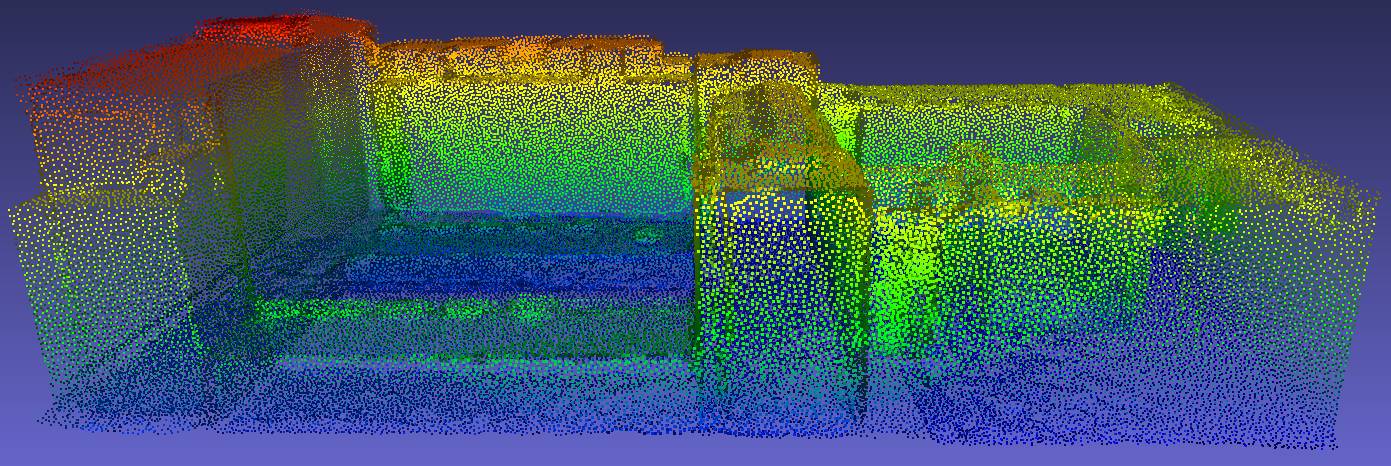
\includegraphics[height=1.5cm]{images/difference_mesh_model/pc_building_bercy}
                            \caption{3D point cloud of a building ($\approx 1.2\mathrm{e}{5}$ points).}
                        \end{center}
                    \end{subfigure}
                    \begin{subfigure}{.45\textwidth}
                        \begin{center}
                            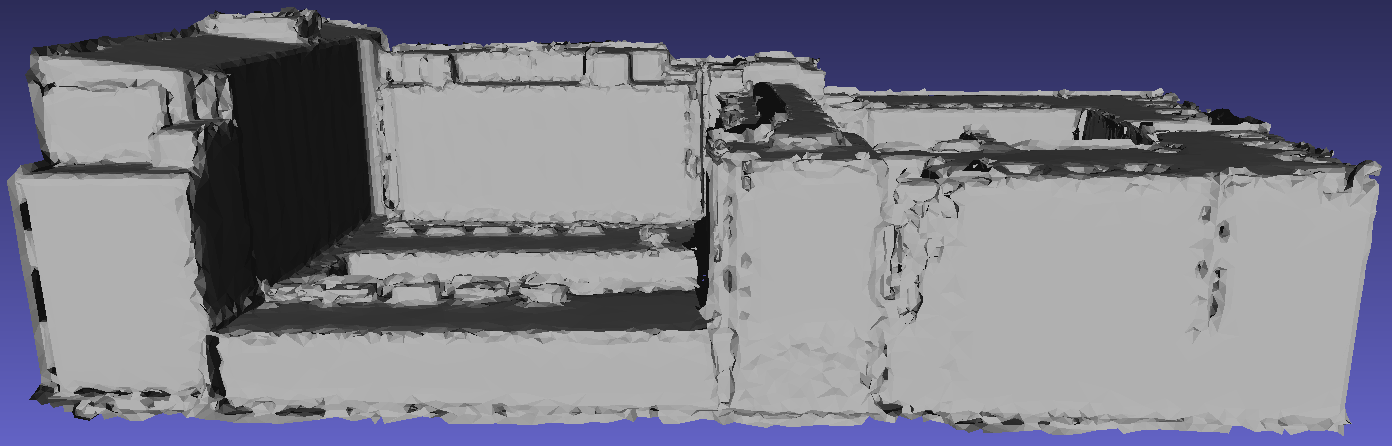
\includegraphics[height=1.5cm]{images/difference_mesh_model/bercy_building_mesh_1_e5}
                            \caption{3D mesh representing a building surface ($\approx 1.0\mathrm{e}{5}$ triangles).}
                        \end{center}
                    \end{subfigure}
                    \\
                    \begin{subfigure}{\textwidth}
                        \begin{center}
                            \includestandalone[mode=buildnew, height=3cm]{ground_truth_model}
                            \caption{Building 3D polyhedral model ($\approx 800$ faces).}
                        \end{center}
                    \end{subfigure}
                \end{center}
            \end{figure}
        \end{frame}
        \begin{frame}{Motivation}
            \only<1-4>{
                \begin{itemize}[label=$\blacktriangleright$, font=\color{IGNGreen}, itemsep=2em]
                    \item<1-> Automatic urban modeling: an active research area~\citep{Musialski2012};
                    \item<2-> Results seamless but lack generality and often erroneous~\citep{rottensteiner2014results};
                    \begin{itemize}[label=$\longrightarrow$]
                        \item<3-> labourious manual corrections.
                    \end{itemize}
                    \item<4-> Urban 3D model semantic diagnostic \textcolor{purple}{not well studied}~\citep{nguatem2017modeling};
                \end{itemize}
            }
            \only<5->{
                \begin{itemize}[label=Goal $\longrightarrow$, font=\color{purple}, leftmargin=2cm]
                    \item<5-> Detect and describe semantic errors that affect building 3D models.
                \end{itemize}
                \begin{itemize}[label=$\blacktriangleright$, font=\color{IGNGreen}, itemsep=2em]
                    \item<6-> Semantic errors independent from \textbf{reconstruction methods} and \textbf{urban scenes}.
                    \item<7-> \textbf{Transferability}, and hence scallability, of the evaluation method.
                \end{itemize}
            }
        \end{frame}
        \begin{frame}{Potential use}
            \begin{itemize}[label=$\blacktriangleright$, font=\color{IGNGreen}, itemsep=2em]
                \item<1-> Change detection;
                \item<2-> Urban models correction;
                \item<3-> Urban reconstruction method evaluation;
                \item<4-> Crowd reconstruction quality assessment.
            \end{itemize}
        \end{frame}

    \section{Methodology}
        \begin{frame}{Main ideas behind our approach}
            \begin{itemize}[label=$\blacktriangleright$, font=\color{IGNGreen}, itemsep=2em]
                \item<1-> Compile errors that affect building models in a taxonomy;
                \item<2-> Evaluation at building level $\Longrightarrow$ formulated as a supervised classification problem;
                \item<3-> Study in a \textbf{2.5D overhead (aerial)} modeling setting.
            \end{itemize}
        \end{frame}
        \begin{frame}{Taxonomy structure}
            Two criteria determine the taxonomy structure:
            \begin{itemize}[label=$\blacktriangleright$, font=\color{IGNGreen}, itemsep=2em]
                \item<2-> the \textbf{\acrfull{acr::lod}};
                \item<3-> the \textbf{\emph{finesse}}: the semantic evaluation level.
            \end{itemize}
            ~\\
            \uncover<4->{
                \begin{block}{Definition}
                    An error is of maximal \emph{finesse} $\Leftrightarrow$ it corresponds, semantically, to a unitary action required to correct the model. The error is called \emph{atomic}.
                \end{block}
            }
        \end{frame}
        \begin{frame}{Error taxonomy (\textit{finesse} $= 0$)}
            \begin{figure}
                \includestandalone[mode=buildnew, height=.7\textheight]{finesse_0_taxonomy}
            \end{figure}
        \end{frame}
        \begin{frame}{Error taxonomy (\textit{finesse} $= 1$)}
            \begin{figure}
                \includestandalone[mode=buildnew, height=.7\textheight]{finesse_1_taxonomy}
            \end{figure}
        \end{frame}
        \begin{frame}{Error taxonomy (\textit{finesse} $= 2$)}
            \begin{figure}
                \includestandalone[mode=buildnew, height=.7\textheight]{finesse_2_taxonomy}
            \end{figure}
        \end{frame}
        \begin{frame}{Error taxonomy (\textit{finesse} $= 2$)}
            \begin{figure}
                \includestandalone[mode=buildnew, height=.7\textheight]{finesse_2_taxonomy_lods}
            \end{figure}
        \end{frame}
        \begin{frame}{Error taxonomy (\textit{finesse} $= 3$)}
            \begin{figure}
                \includestandalone[mode=buildnew, width=\textwidth]{finesse_3_bul_taxonomy}
            \end{figure}
        \end{frame}
        \begin{frame}{Building \textit{atomic} errors: 2.5D overhead reconstruction case}
            \begin{figure}
                \begin{center}
                    \begin{subfigure}{.28\textwidth}
                        \fbox{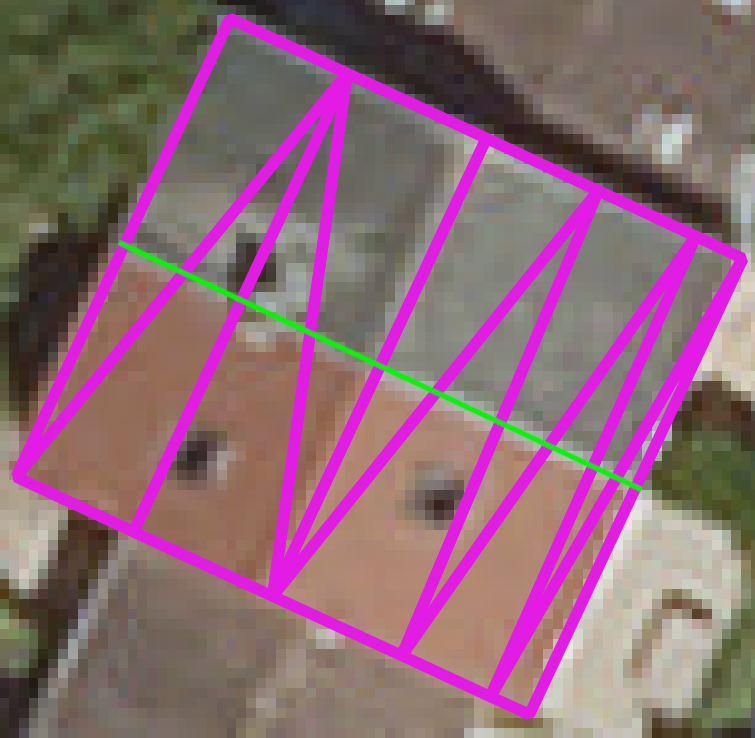
\includegraphics[height=1.75cm]{images/errors/building/under_segmentation}}
                        \caption{\label{fig::bul_under} Under segmentation}
                    \end{subfigure}
                    \begin{subfigure}{.28\textwidth}
                        \fbox{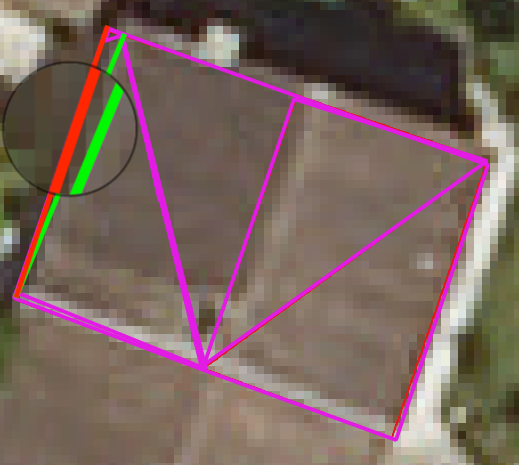
\includegraphics[height=1.75cm]{images/errors/building/border}}
                        \caption{\label{fig::bul_footprint} Imprecise border}
                    \end{subfigure}
                    \begin{subfigure}{.28\textwidth}
                        \fbox{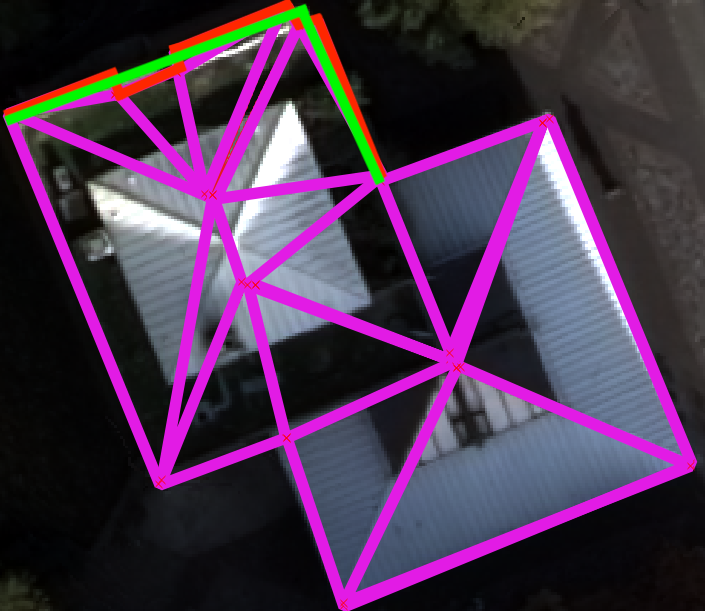
\includegraphics[height=1.75cm]{images/errors/building/topology}}
                        \caption{\label{fig::bul_height} Inaccurate topology}
                    \end{subfigure}
                    \begin{subfigure}{.33\textwidth}
                        \fbox{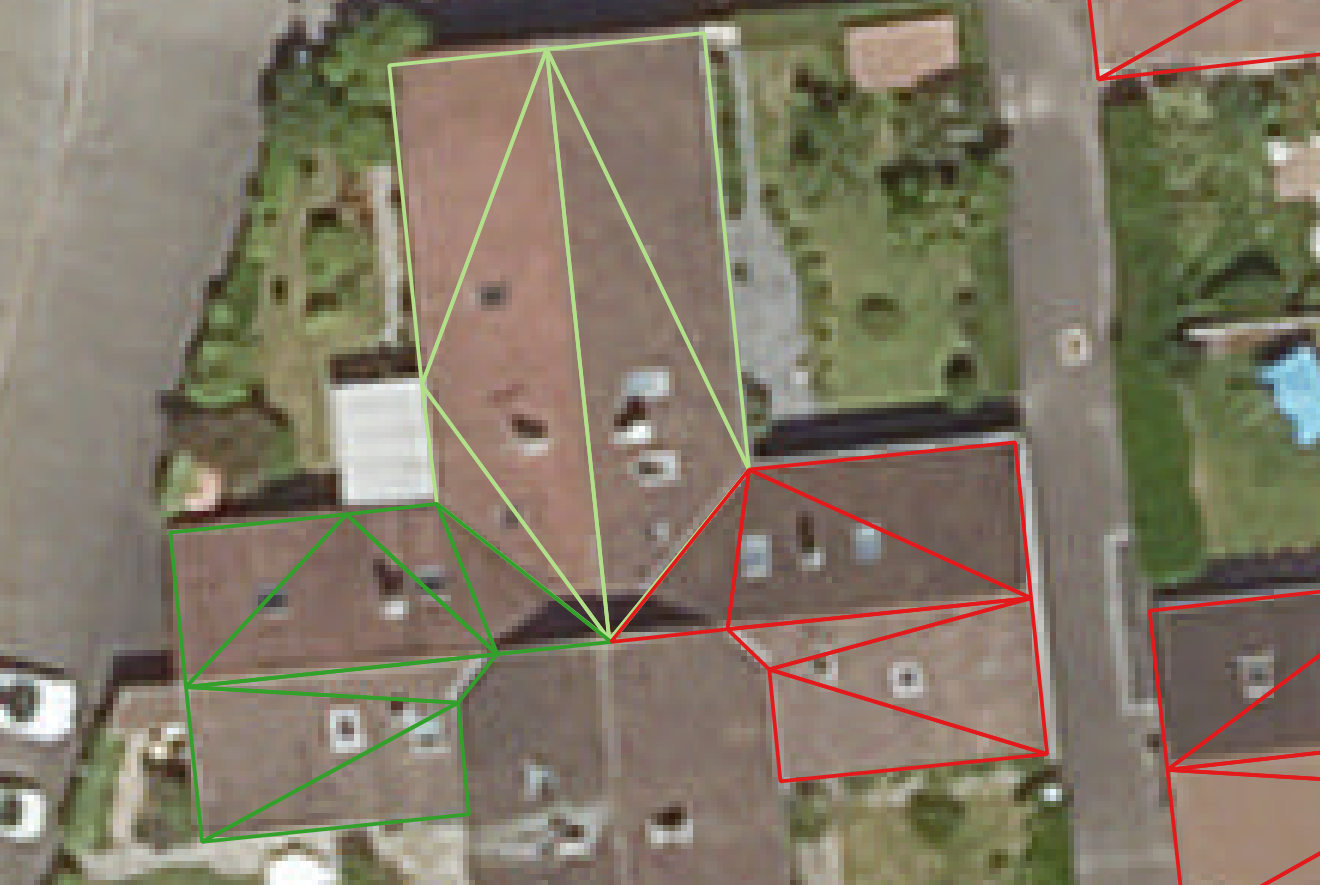
\includegraphics[height=2cm]{images/errors/building/over_segmentation}}
                        \caption{\label{fig::bul_over} Over segmentation}
                    \end{subfigure}
                \end{center}
            \end{figure}
        \end{frame}
        \begin{frame}{Error taxonomy (\textit{finesse} $= 3$)}
            \begin{figure}
                \includestandalone[mode=buildnew, width=\textwidth]{finesse_3_all_taxonomy}
            \end{figure}
        \end{frame}
        \begin{frame}{Facet \textit{atomic} errors: 2.5D overhead reconstruction case}
            \begin{figure}
                \begin{center}
                    \begin{subfigure}{.28\textwidth}
                        \fbox{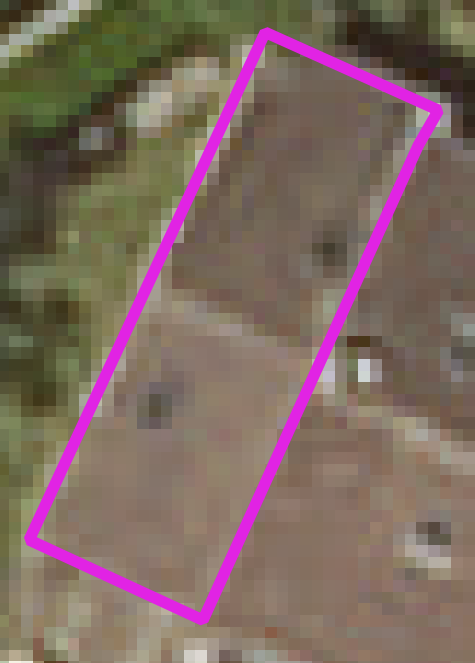
\includegraphics[height=2cm]{images/errors/facet/under_segmentation}}
                        \caption{\label{fig::fac_under} Under segmentation}
                    \end{subfigure}
                    \begin{subfigure}{.28\textwidth}
                        \fbox{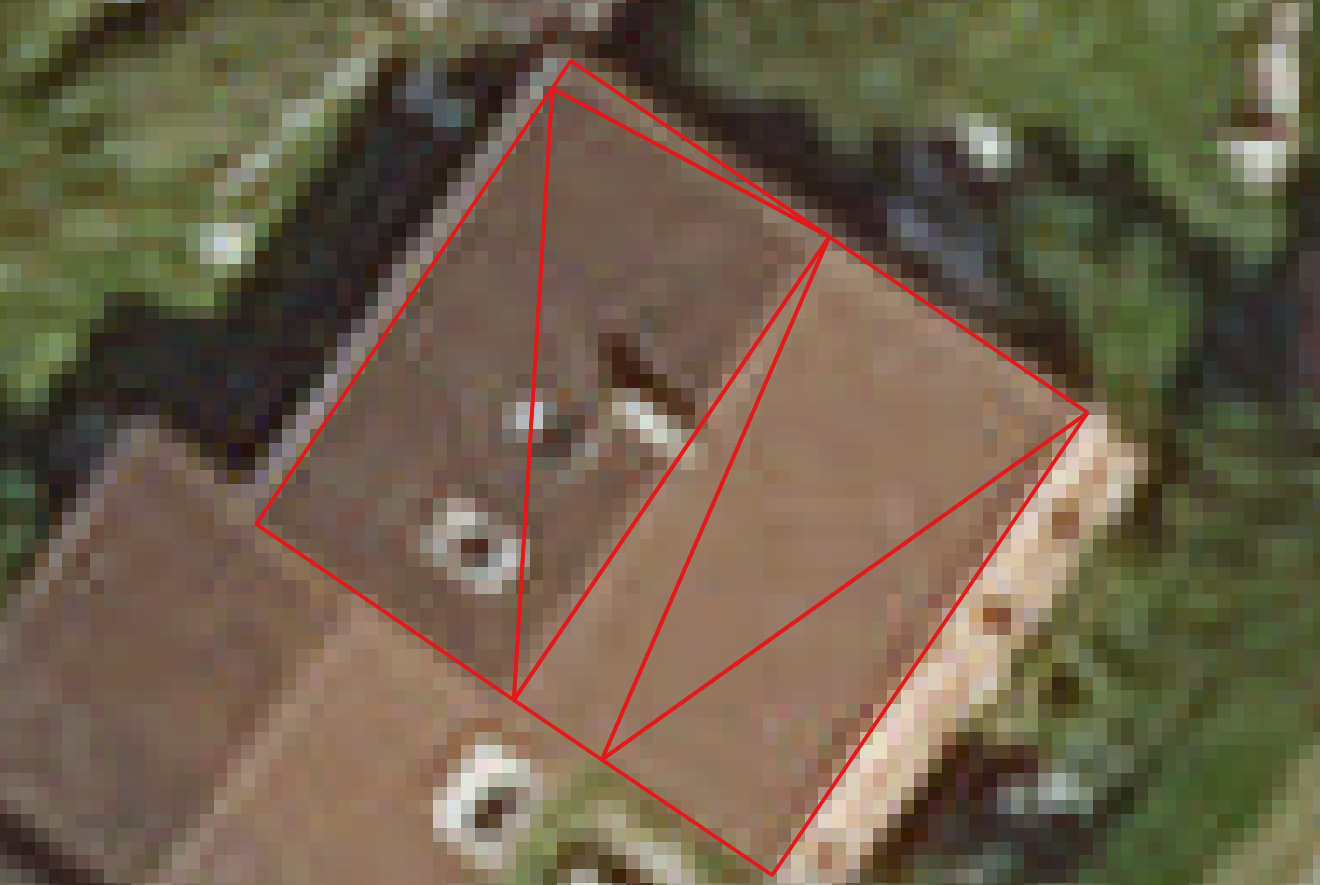
\includegraphics[height=2cm]{images/errors/facet/over_segmentation}}
                        \caption{\label{fig::fac_over} Over segmentation}
                    \end{subfigure}
                    \begin{subfigure}{.28\textwidth}
                        \fbox{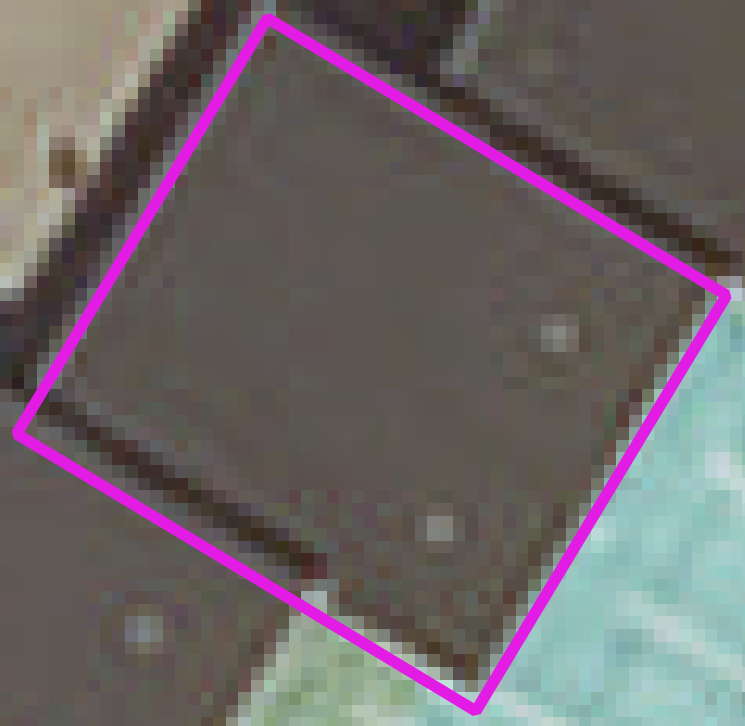
\includegraphics[height=2cm]{images/errors/facet/geometry}}
                        \caption{\label{fig::fac_height} Imprecise geometry}
                    \end{subfigure}
                    \begin{subfigure}{.33\textwidth}
                        \fbox{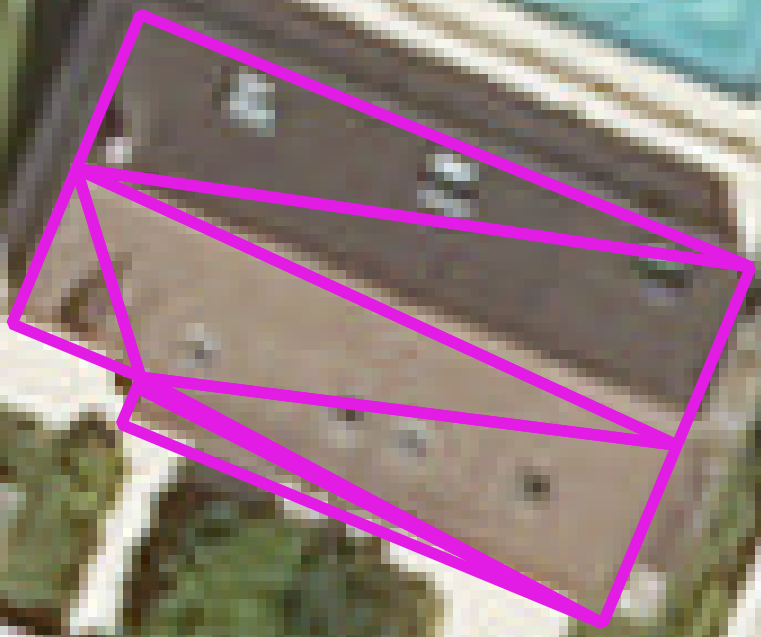
\includegraphics[height=2cm]{images/errors/facet/border}}
                        \caption{\label{fig::fac_footprint} Imprecise borders}
                    \end{subfigure}
                    \begin{subfigure}{.33\textwidth}
                        \fbox{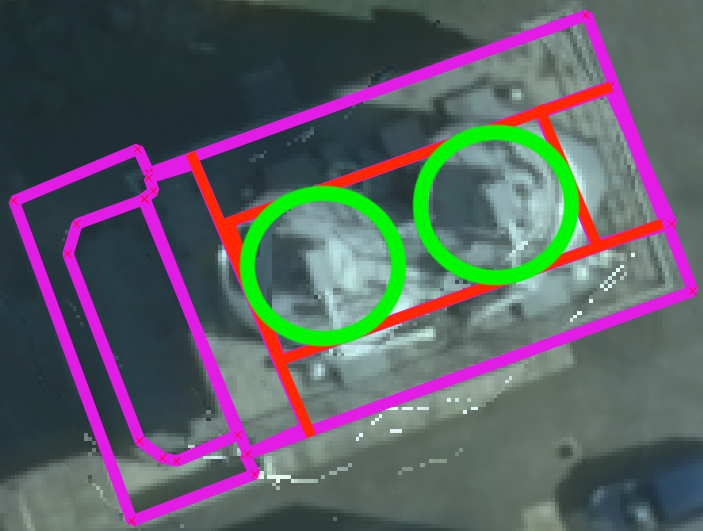
\includegraphics[height=2cm]{images/errors/facet/topology}}
                        \caption{\label{fig::fac_height} Inaccurate topology}
                    \end{subfigure}
                \end{center}
            \end{figure}
        \end{frame}
        \subsection{Quality prediction pipeline}
            \begin{frame}{The evaluation pipeline}
                \begin{figure}
                    \includegraphics[width=\textwidth]{graphical_abstract}
                \end{figure}
            \end{frame}
\end{document}